%%%%%%%%%%%%%%%%%%%%%%%%%%%%%%%%%%%%%%%%%%%%%%%%%%%%%%%%%%%%
%%% ELIFE ARTICLE TEMPLATE
%%%%%%%%%%%%%%%%%%%%%%%%%%%%%%%%%%%%%%%%%%%%%%%%%%%%%%%%%%%%
%%% PREAMBLE 
\documentclass[9pt,lineno,final]{elife}
% Use the onehalfspacing option for 1.5 line spacing
% Use the doublespacing option for 2.0 line spacing
% Please note that these options may affect formatting.
% Additionally, the use of the \newcommand function should be limited.

% Article specific functions
\newcommand{\pKa}{p\textit{K}\textsubscript{a}}
\newcommand{\psKa}{p\textsubscript{s}\textit{K}\textsubscript{a}}


\usepackage{lipsum} % Required to insert dummy text
\usepackage[version=4]{mhchem}
%\usepackage{siunitx}
%\DeclareSIUnit\Molar{M}
\usepackage[colorinlistoftodos]{todonotes}
\usepackage{gensymb}
\usepackage{mhchem}
\usepackage{wrapfig}
\usepackage{booktabs}
\usepackage[flushleft]{threeparttable}
%\usepackage{longtable} % for tables that are longer than one page
\usepackage{float}

% some tint of orange
\definecolor{tangelo}{rgb}{0.98, 0.3, 0.0}
% var for storing a box size
\newsavebox{\measurebox}

% Hidden table column
%\newcolumntype{H}{>{\setbox0=\hbox\bgroup}c<{\egroup}@{}}

% For having Supplemantary Information Section in the same document
\newcommand{\beginsupplement}{%
        \setcounter{table}{0}
        \renewcommand{\thetable}{S\arabic{table}}%
        \setcounter{figure}{0}
        \renewcommand{\thefigure}{S\arabic{figure}}%
     }
     
% To have landscape pages
\usepackage{pdflscape}

% For color coded to-do and comment bubbles
\newcommand{\todoMI}[1]{\todo[inline, author=MI, color=blue!20]{ #1}}


%%%%%%%%%%%%%%%%%%%%%%%%%%%%%%%%%%%%%%%%%%%%%%%%%%%%%%%%%%%%
%%% ARTICLE SETUP
%%%%%%%%%%%%%%%%%%%%%%%%%%%%%%%%%%%%%%%%%%%%%%%%%%%%%%%%%%%%
\title{Accuracy of macroscopic and microscopic \pKa{} predictions of small molecules evaluated by the SAMPL6 blind prediction challenge}

\author[1,2*]{Mehtap Işık (ORCID: \href{http://orcid.org/0000-0002-6789-952X}{0000-0002-6789-952X})}
\author[1,3]{Ari\"{e}n S. Rustenburg (ORCID: \href{http://orcid.org/0000-0002-3422-0613}{0000-0002-3422-0613})}
\author[1,4]{Andrea Rizzi (ORCID: \href{https://orcid.org/0000-0001-7693-2013}{0000-0001-7693-2013})}
\author[6]{M. R. Gunner} % Marilyn wants to be "M. R. Gunner"
\author[5]{David L. Mobley (ORCID: \href{http://orcid.org/0000-0002-1083-5533}{0000-0002-1083-5533})}
\author[1]{John D. Chodera (ORCID: \href{http://orcid.org/0000-0003-0542-119X}{0000-0003-0542-119X})}

\affil[1]{Computational and Systems Biology Program, Sloan Kettering Institute, Memorial Sloan Kettering Cancer Center, New York, NY 10065, United States}
\affil[2]{Tri-Institutional PhD Program in Chemical Biology, Weill Cornell Graduate School of Medical Sciences, Cornell University, New York, NY 10065, United States}
\affil[3]{Graduate Program in Physiology, Biophysics, and Systems Biology, Weill Cornell Medical College, New York, NY 10065, United States}
\affil[4]{Tri-Institutional PhD Program in Computational Biology and Medicine, Weill Cornell Graduate School of Medical Sciences, Cornell University, New York, NY 10065, United States}
\affil[5]{Department of Pharmaceutical Sciences and Department of Chemistry, University of California,
Irvine, Irvine, California 92697, United States}
\affil[6]{Department of Physics, City College of New York, New York NY 10031}

\corr{mehtap.isik@choderalab.org}{MI}

%%%%%%%%%%%%%%%%%%%%%%%%%%%%%%%%%%%%%%%%%%%%%%%%%%%%%%%%%%%%
%%% ARTICLE START
%%%%%%%%%%%%%%%%%%%%%%%%%%%%%%%%%%%%%%%%%%%%%%%%%%%%%%%%%%%%

\begin{document}

\maketitle

%%%%%%%%%%%%%%%%%%%%%%%%%%%%%%%%%%%%%%%%%%%%%%%%%%%%%%%%%%%%
% Abstract
%%%%%%%%%%%%%%%%%%%%%%%%%%%%%%%%%%%%%%%%%%%%%%%%%%%%%%%%%%%%
\begin{abstract}
\todo[inline]{Complete abstract.}
- number of submissions~\cite{Isik:2018:J.Comput.AidedMol.Des.}

- summary of analysis  

- difficulties observed  

\end{abstract}

%%%%%%%%%%%%%%%%%%%%%%%%%%%%%%%%%%%%%%%%%%%%%%%%%%%%%%%%%%%%
% Keywords and Abbreviations
%%%%%%%%%%%%%%%%%%%%%%%%%%%%%%%%%%%%%%%%%%%%%%%%%%%%%%%%%%%%
\subsection{Keywords}
SAMPL $\cdot$ blind prediction challenge $\cdot$ acid dissociation constant $\cdot$ \pKa{} $\cdot$ small molecule $\cdot$ macroscopic \pKa $\cdot$ microscopic \pKa  $\cdot$ macroscopic protonation state $\cdot$ microscopic protonation state

\subsection{Abbreviations}
\begin{description}
\item[SAMPL] Statistical Assessment of the Modeling of Proteins and Ligands
\item[\pKa]  --${\log_{10}}$ acid dissociation equilibrium constant 
\item[SEM] Standard error of the mean
\item[RMSE] Root mean squared error
\item[MAE] Mean absolute error
\item[{$\tau$}] Kendall's rank correlation coefficient (Tau)
\item[R\textsuperscript{2}] Coefficient of determination (R-Squared)
\end{description}


%%%%%%%%%%%%%%%%%%%%%%%%%%%%%%%%%%%%%%%%%%%%%%%%%%%%%%%%%%%%
% Introduction
%%%%%%%%%%%%%%%%%%%%%%%%%%%%%%%%%%%%%%%%%%%%%%%%%%%%%%%%%%%%
\section{Introduction}
\todo[inline]{Complete introduction section:
- Importance of small molecule pKa prediction for pharmaceutical efforts. 
- Definition of pKa  
- Acid dissociation equilibrium constant  
- Add pKa equation  
- Add free energy of protonation state equation  
- Definition of microscopic and macroscopic pKas  
- Introduce linear protonation state free energy diagram [Cite Gunner et al 2019 paper]  
FIGURE: linear plot of free energy vs pH  
}

\todo[inline]{Importance of small molecule pKa prediction for pharmaceutical efforts.}

\todo[inline]{Explain why we are doing a pKa challenge and connect to past and previous challenges}
SAMPL (Statistical Assessment of the Modeling of Proteins and Ligands). About SAMPL challenges: Collectively, these challenges have assessed the effects of force field accuracy, solvation models, pKa and tautomer predictions.  

During the SAMPL5 challenge, log D predictions experienced difficulties predicting log D values accurately, unless protonation states and tautomers were taken into account.

For this iteration of the SAMPL challenge, we have taken one step back and isolated just the problem of predicting solvent protonation states.

This is the first time a blind pKa prediction challenge has been fielded as part of SAMPL. 
In this first iteration of the challenge, we aimed to assess the performance of current pKa prediction methods and isolate potential causes of inaccurate pKa estimates, with the aim of determining how pKa prediction inaccuracies might impact predicted affinities for drug-like molecules. 
For example, for both logD and binding affinity predictions, any error in predicting the free energy of accessing a minor protonation state in solution that becomes dominant in the complex will directly add to the error in the predicted transfer or binding free energy. 

Challenge goal: determining how pKa prediction inaccuracies might impact predicted affinities for drug-like molecules. For example, for both logD and binding affinity predictions, any error in predicting the free energy of accessing a minor protonation state in solution that becomes dominant in the complex will directly add to the error in the predicted transfer or binding free energy. 

Reason for blind pKa challenge:
- Impact on binding affinity predictions
- Impact on logD predictions (SAMPL6)
- Drug-like molecules are especially challenging.

Protonation state effects were a dominant accuracy-limiting factor for logD from SAMPL5, and should also be accuracy-limiting in binding free energy predictions.
Errors is \pKa{} predictions can cause modeling the wrong charge, protonation and tautomerization states which affect hydrogen bonding opportunities and overall dipole moment of the ligand.

\todo[inline]{Explain the physics of the predicted property}
\todo[inline]{EQUATION: pKa equation}
\todo[inline]{EQUATION: free energy of protonation state equation}
\todo[inline]{Introducing linear protonation state free energy diagram}
\todo[inline]{FIGURE: linear plot of free energy vs pH }

\todo[inline]{FIGURE: a diagram illustrating the ways in which the pKa errors can influence prediction errors for binding affinities}

\todo[inline]{Overview of kinds of pKa prediction methods available  (ML, QM, empirical methods ... }

\todo[inline]{Explain challenge design.}

Experimental macroscopic pKa values were measured using a UV-metric assay performed using a Sirius T3 [cite exp. paper ]  supported by Merck, MRL,  Rahway NJ.  

\begin{figure}
\begin{center}
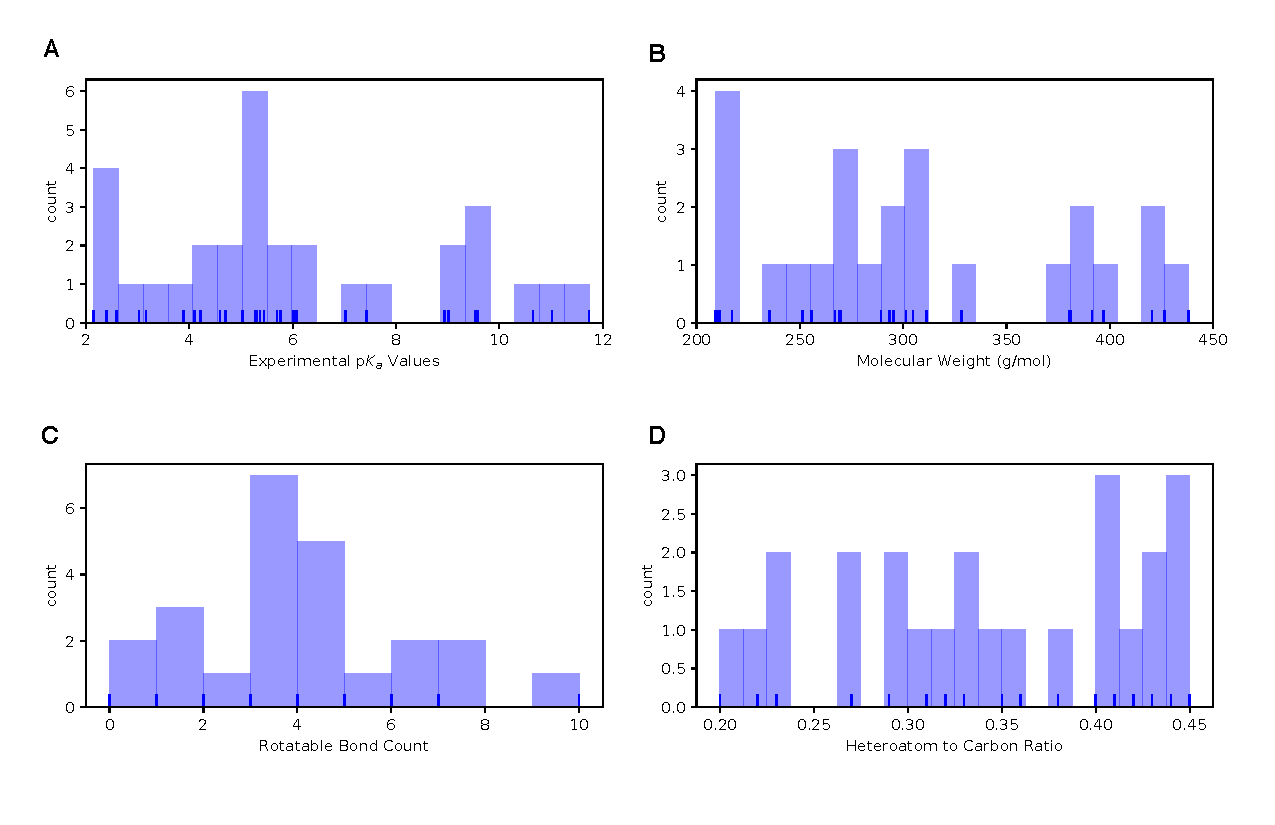
\includegraphics[width=1.0\linewidth]{figures/distribution_of_molecular_properties.pdf}
\caption{{\bf Distribution of molecular properties of 24 compounds in SAMPL6 \pKa{} Challenge.} {\bf A} Histogram of spectrophotometric \pKa{} measurements collected with Sirius T3 ~\cite{Isik:2018:J.Comput.AidedMol.Des.}. Overlayed carpet plot indicates the actual values. Five compounds have multiple measured \pKa{}s in the range of 2-12. {\bf B} Histogram of molecular weights of compounds in SAMPL6 set. Molecular weights were calculated by neglecting counter ions. {\bf C} Histogram of the number of non-terminal rotatable bonds in each molecule. {\bf D} The histogram of the ratio of heteroatom (non-carbon heavy atom) count to the number of carbon atoms.
}
\label{fig:dist_mol_prop}
\end{center}
\end{figure}

Communicate concepts behind challenge design and why we made specific choices:
Explain why we have types I, II, III
Explain why we preenumerated microstates

Participants had the option to submit predictions in one of 3 categories: Microscopic pKa values (type I), microscopic state populations (type II), or macroscopic pKa values (type III).

The comparison between macroscopic and microscopic pKa values is not always a straightforward one. 

Overview of available pKa prediction methods and methods that participated in SAMPL6. [Reminder to cite all papers here.]

\todo[inline]{Explain future direction for this challenge}
Challenge path: predict pKas, give people pKas to predict logDs on same molecules, then predict for new set of compounds logDs without provided pKas.
\todo[inline]{Explain potantial benefits of these challenge}
Improving computational methods...


%%%
\subsection{Motivation for a blind pKa challenge}

why we are doing a pKa challenge and connect to past and previous challenge?

SAMPL (Statistical Assessment of the Modeling of Proteins and Ligands). About SAMPL challenges: Collectively, these challenges have assessed the effects of force field accuracy, solvation models, pKa and tautomer predictions.  

During the SAMPL5 challenge, log D predictions experienced difficulties predicting log D values accurately, unless protonation states and tautomers were taken into account.

For this iteration of the SAMPL challenge, we have taken one step back and isolated just the problem of predicting solvent protonation states.

This is the first time a blind pKa prediction challenge has been fielded as part of SAMPL. 
In this first iteration of the challenge, we aimed to assess the performance of current pKa prediction methods and isolate potential causes of inaccurate pKa estimates, with the aim of determining how pKa prediction inaccuracies might impact predicted affinities for drug-like molecules. 
For example, for both logD and binding affinity predictions, any error in predicting the free energy of accessing a minor protonation state in solution that becomes dominant in the complex will directly add to the error in the predicted transfer or binding free energy. 

Challenge goal: determining how pKa prediction inaccuracies might impact predicted affinities for drug-like molecules. For example, for both logD and binding affinity predictions, any error in predicting the free energy of accessing a minor protonation state in solution that becomes dominant in the complex will directly add to the error in the predicted transfer or binding free energy. 

Reason for blind pKa challenge:  
1. Impact on binding affinity predictions  
2. Impact on logD predictions (SAMPL6)  
3.  Drug-like molecules are especially challenging.  


Future challenge direction  
Challenge path: predict pKas, give people pKas to predict logDs on same molecules, then predict for new set of compounds logDs without provided pKas.  
Potantial benefits of these challenges:  
1. Improving computational methods  
2. Detecting hidden contributors to error  

%%%
\subsection{Approaches to predict pKas}

Overview of kinds of pKa prediction methods available  (ML, QM, empirical methods ... 


%%%%%%%%%%%%%%%%%%%%%%%%%%%%%%%%%%%%%%%%%%%%%%%%%%%%%%%%%%%%
% Methods
%%%%%%%%%%%%%%%%%%%%%%%%%%%%%%%%%%%%%%%%%%%%%%%%%%%%%%%%%%%%
\section{Methods}

%%%
\subsection{Structure and logistics of the SAMPL6 pKa prediction challenge}
\todo[inline]{Describe the structure of SAMPL6 pKa challenge}

Experimental macroscopic pKa values were measured using a UV-metric assay performed using a Sirius T3 [cite exp. paper ]  supported by Merck, MRL,  Rahway NJ.

Communicate concepts behind challenge design and why we made specific choices:  
1. Explain why we have types I, II, III  
2. Explain why we pre-enumerated microstates  


Participants had the option to submit predictions in one of 3 categories: Microscopic pKa values (type I), microscopic state populations (type II), or macroscopic pKa values (type III).

The comparison between macroscopic and microscopic pKa values is not always a straightforward one. 

- When instructions and input files were made available

- Challenge dates

- Input files

- What to predict? Three type of submissions.

- Multiple submissions allowed

- Predicting the pKa values of the whole set wasn't a requirement. 

- 2nd D3R/SAMPL Workshop took place in La Jolla, San Diego on Feb 22-23, 2018.

Referece Figure \ref{fig:dist_exp_pKas}. Drug-like molecules are often larger and more complex than the ones used in this study.


%%%
\subsection{Enumeration of requested prediction microscopic protonation states}
1. OpenEye (filter out resonance structures), Epik  

2. Participant supplied structures  

Microstate pairs: Only +/-1 charge change transitions are allowed.
List of allowed transitions. +2 transitions are not considered.


%%%
\subsection{Evaluation approaches}

\subsubsection{Statistical metrics for submission performance}

- Root mean squared error (RMSE)

- Mean absolute error (MAE)

- Mean Error (ME)

- Square of Pearson Correlation Coefficient (R\textsuperscript{2})

- Slope of prediction vs. experimental value linear fit

Uncertainty in each performance statistic was calculated by bootstapping (10,000) to estimate 95\% confidence intervals.

\subsubsection{Matching algorithms for pairing predicted and experimental pKas}

Explain why it is necessary due to lacking structural information. Cite recommendations from article such as preserving sequence.
Experimental data doesn't inform protonation site and overall charge of species.
 Experimental data doesn't capture the whole picture. We don't know charge and we don't know tautomers.
 We don't know the charge state of macrostates, this causes a matching problem


Explain Hungarian method for matching experimental and predicted pKas

Explain Closest method for matching experimental and predicted pKas

Explain microstate based matching.


%%%
\subsection{Reference calculations}

Schrodinger Epik
Schrodinger Jaguar
Chemicalize
MoKa


%%%%%%%%%%%%%%%%%%%%%%%%%%%%%%%%%%%%%%%%%%%%%%%%%%%%%%%%%%%%
% Results and Discussion
%%%%%%%%%%%%%%%%%%%%%%%%%%%%%%%%%%%%%%%%%%%%%%%%%%%%%%%%%%%%
\section{Results and Discussion}

\todo[inline]{A paragraph to explain the submission methods. Define method categories: DL, LFER, QSPR/ML, QM, QM+LEC, and QM+MM, Blind predictions, Reference calculations, Null model (pKa prospector lookup)
}
\todoMI{TABLE: Table [method-names-and-submission-IDs]. Submissions spanning different method categories were made to the SAMPL6 pKa Challenge: DL, LFER, QSPR/ML, QM, QM+LEC, and QM+MM. Unique submission IDs were assigned to each submission even for different submission types (I, II, or III) when multiple submissions were made for the same method. }







\begin{table}%[H]%[tb!]
\begin{center}
\begin{threeparttable}
\centering\scriptsize
\caption{{\bf Submission IDs, names, category, and type for all the \pKa{} prediction sets.} 
Reference calculations are labeled as \textit{nb\#\#\#}. The method name column lists the names provided by each participant in the submission file. The ``type'' column indicates if submission was or a post-deadline reference calculation, denoted by ``Blind'' or ``Reference'' respectively. The table is not ordered by performance.  
} 
\label{submission-ID-table}
\begin{tabular}{@{}llllll@{}}
\toprule
\textbf{\begin{tabular}[c]{@{}l@{}}Method \\ Category\end{tabular}} & \textbf{Method} & \textbf{\begin{tabular}[c]{@{}l@{}}Microscopic \pKa{} \\ (Type I) \\ Submission ID\end{tabular}} & \textbf{\begin{tabular}[c]{@{}l@{}}Macroscopic \pKa{} \\ (Type III) \\ Submission ID\end{tabular}} & \textbf{\begin{tabular}[c]{@{}l@{}}Submission \\ Type\end{tabular}} & \textbf{References} \\ \midrule
DL & Substructure matches to experimental data in pKa OpenEye pKa Prospector Database v1.0 & \textit{} & \textit{5nm4j} & Null & \cite{pKa-prospector-ref} \\
DL & OpenEye pKa-Prospector 1.0.0.3 with Analog Search ion identification algorithm & \textit{} & \textit{pwn3m} & Blind & \cite{pKa-prospector-ref} \\
LFER & ACD/pKa GALAS (ACD/Percepta Kernel v1.6) & \textit{v8qph} & \textit{37xm8} & Blind & \cite{ACD-pKa-galas} \\
LFER & ACD/pKa Classic (ACD/Percepta Kernel, v1.6) & \textit{} & \textit{xmyhm} & Blind & \cite{ACD-pKa-classic} \\
LFER & Epik Scan (Schrodinger v2017-4) & \textit{} & \textit{nb007} & Reference & \cite{Shelley:2007:J.Comput.AidedMol.Des.} \\
LFER & Epik Microscopic (Schrodinger v2017-4) & \textit{nb008} & \textit{nb010} & Reference & \cite{Shelley:2007:J.Comput.AidedMol.Des.} \\
QSPR/ML & OpenEye Gaussian Process & \textit{6tvf8} & \textit{hytjn} & Blind & \cite{Bannan:2018:J.Comput.AidedMol.Des.} \\
QSPR/ML & OpenEye Gaussian Process Resampled & \textit{} & \textit{q3pfp} & Blind & \cite{Bannan:2018:J.Comput.AidedMol.Des.} \\
QSPR/ML & S+pKa (ADMET Predictor v8.5, Simulations Plus) & \textit{hdiyq} & \textit{gyuhx} & Blind & \cite{simulation-plus-pKa} \\
QSPR/ML & Chemicalize v18.23 (ChemAxon MarvinSketch v18.23) & \textit{} & \textit{nb015} & Reference & \cite{chemicalize-pKa} \\
QSPR/ML & MoKa v3.1.3 & \textit{nb016} & \textit{nb017} & Reference & \cite{Milletti:2007:J.Chem.Inf.Model., moka-pKa} \\
QM & \begin{tabular}[c]{@{}l@{}}Adiabatic scheme with single point correction:  SMD/M06-2X//6-311++G(d,p)//M06-2X/6-31+G(d) \\ for bases and SMD/M06-2X//6-311++G(d,p)//M06-2X/6-31G(d) for acids  + thermal corrections\end{tabular} & \textit{ko8yx} & \textit{ryzue} & Blind & \cite{Zeng:2018:J.Comput.AidedMol.Des.} \\
QM & \begin{tabular}[c]{@{}l@{}}Direct scheme with single point correction: SMD/M06-2X//6-311++G(d,p)//M06-2X/6-31+G(d) for \\ bases and SMD/M06-2X//6-311++G(d,p)//M06-2X/6-31G(d) for acids  + thermal corrections\end{tabular} & \textit{w4z0e} & \textit{xikp8} & Blind & \cite{Zeng:2018:J.Comput.AidedMol.Des.} \\
QM & \begin{tabular}[c]{@{}l@{}}Adiabatic scheme: thermodynamic cycle that uses gas phase optimized structures for gas phase free \\ energy and solution phase geometries for solvent phase free energy. SMD/M06-2X/6-31+G(d) for \\ bases and SMD/M06-2X/6-31G(d) for acids + thermal corrections\end{tabular} & \textit{wcvnu} & \textit{5byn6} & Blind & \cite{Zeng:2018:J.Comput.AidedMol.Des.} \\
QM & \begin{tabular}[c]{@{}l@{}}Vertical scheme:  thermodynamic cycle that uses only gas phase optimized structures to compute gas \\ hase and solvation free energy. SMD/M06-2X/6-31+G(d) for bases and SMD/M06-2X/6-31G(d) for \\ acids + Thermal corrections\end{tabular} & \textit{arcko} & \textit{w4iyd} & Blind & \cite{Zeng:2018:J.Comput.AidedMol.Des.} \\
QM & \begin{tabular}[c]{@{}l@{}}Direct scheme: solution phase free energy is determined by solution phase geometries  without \\ thermodynamic cycle SMD/M06-2X/6-31+G(d) for bases and SMD/M06-2X/6-31G(d) for acids \\ + thermal corrections\end{tabular} & \textit{wexjs} & \textit{y75vj} & Blind & \cite{Zeng:2018:J.Comput.AidedMol.Des.} \\
QM + LEC & Jaguar (Schrodinger v2017-4) & \textit{nb011} & \textit{nb013} & Reference & \cite{Bochevarov:2013:Int.J.QuantumChem.} \\
QM + LEC & CPCM/B3LYP/6–311+G(d,p) and global fitting & \textit{y4wws} & \textit{35bdm} & Blind & \cite{Selwa:2018:J.Comput.AidedMol.Des.} \\
QM + LEC & \begin{tabular}[c]{@{}l@{}}CPCM/B3LYP/6–311+G(d,p) and separate fitting for neutral to negative and for positive to neutral \\ transformations\end{tabular} & \textit{qsicn} & \textit{p0jba} & Blind & \cite{Selwa:2018:J.Comput.AidedMol.Des.} \\
QM + LEC & EC-RISM/MP2/6-311+G(d,p)-P3NI-q-noThiols-2par & \textit{kxztt} & \textit{ds62k} & Blind & \cite{Tielker:2018:J.Comput.AidedMol.Des.} \\
QM + LEC & EC-RISM/MP2/cc-pVTZ-P2-q-noThiols-2par & \textit{ftc8w} & \textit{2ii2g} & Blind & \cite{Tielker:2018:J.Comput.AidedMol.Des.} \\
QM + LEC & EC-RISM/MP2/6-311+G(d,p)-P2-phi-all-2par & \textit{ktpj5} & \textit{nb001} & Blind* & \cite{Tielker:2018:J.Comput.AidedMol.Des.} \\
QM + LEC & EC-RISM/MP2/6-311+G(d,p)-P2-phi-noThiols-2par & \textit{wuuvc} & \textit{nb002} & Blind* & \cite{Tielker:2018:J.Comput.AidedMol.Des.} \\
QM + LEC & EC-RISM/MP2/6-311+G(d,p)-P3NI-phi-all-2par & \textit{2umai} & \textit{nb003} & Blind* & \cite{Tielker:2018:J.Comput.AidedMol.Des.} \\
QM + LEC & EC-RISM/MP2/6-311+G(d,p)-P3NI-phi-noThiols-2par & \textit{cm2yq} & \textit{nb004} & Blind* & \cite{Tielker:2018:J.Comput.AidedMol.Des.} \\
QM + LEC & EC-RISM/MP2/6-311+G(d,p)-P2-phi-all-1par & \textit{z7fhp} & \textit{nb005} & Blind* & \cite{Tielker:2018:J.Comput.AidedMol.Des.} \\
QM + LEC & EC-RISM/MP2/6-311+G(d,p)-P3NI-phi-all-1par & \textit{8toyp} & \textit{nb006} & Blind* & \cite{Tielker:2018:J.Comput.AidedMol.Des.} \\
QM + LEC & EC-RISM/MP2/cc-pVTZ-P2-phi-noThiols-2par & \textit{epvmk} & \textit{ttjd0} & Blind & \cite{Tielker:2018:J.Comput.AidedMol.Des.} \\
QM + LEC & EC-RISM/MP2/cc-pVTZ-P2-phi-all-2par & \textit{xnoe0} & \textit{mkhqa} & Blind & \cite{Tielker:2018:J.Comput.AidedMol.Des.} \\
QM + LEC & EC-RISM/MP2/cc-pVTZ-P3NI-phi-noThiols-2par & \textit{4o0ia} & \textit{mpwiy} & Blind & \cite{Tielker:2018:J.Comput.AidedMol.Des.} \\
QM + LEC & EC-RISM/B3LYP/6-311+G(d,p)-P3NI-q-noThiols-2par & \textit{nxaaw} & \textit{ad5pu} & Blind & \cite{Tielker:2018:J.Comput.AidedMol.Des.} \\
QM + LEC & EC-RISM/B3LYP/6-311+G(d,p)-P3NI-phi-noThiols-2par & \textit{0xi4b} & \textit{f0gew} & Blind & \cite{Tielker:2018:J.Comput.AidedMol.Des.} \\
QM + LEC & EC-RISM/B3LYP/6-311+G(d,p)-P2-phi-noThiols-2par & \textit{cywyk} & \textit{np6b4} & Blind & \cite{Tielker:2018:J.Comput.AidedMol.Des.} \\
QM + LEC & PCM/B3LYP/6-311+G(d,p) & \textit{gdqeg} & \textit{yc70m} & Blind & \cite{Tielker:2018:J.Comput.AidedMol.Des.} \\
QM + LEC & COSMOtherm\_FINE17 (COSMOtherm C30\_1701, BP/TZVPD/FINE//BP/TZVP/COSMO) & \textit{t8ewk} & \textit{0hxtm} & Blind & \cite{Klamt:2003:J.Phys.Chem.Ab, Eckert:2006:J.Comput.Chem.} \\
QM + LEC & \begin{tabular}[c]{@{}l@{}}DSD-BLYP-D3(BJ)/def2-TZVPD//PBEh-3c[DCOSMO-RS] + RRHO(GFN-xTB[GBSA]) \\ + Gsolv(COSMO-RS[TZVPD]) and linear fit\end{tabular} & \textit{} & \textit{xvxzd} & Blind & \cite{Pracht:2018:J.Comput.AidedMol.Des.} \\
QM + LEC & \begin{tabular}[c]{@{}l@{}}ReSCoSS conformations // DSD-BLYP-D3 reranking // COSMOtherm pKa:  DSD-BLYP-D3(BJ)/\\ def2-TZVPD// PBE-D3(BJ)/def2-TZVP/COSMO + RRHO[GFN-xTB + GBSA-water] \\ + Gsolv[COSMO-RS(FINE17/TZVPD)] level and COSMOtherm pKa applied  at the single conformer \\ pair level  (COSMOthermX17.0.5 release and BP-TZVPD-FINE-C30-1701 parameterization)\end{tabular} & \textit{eyetm} & \textit{8xt50} & Blind & \cite{Pracht:2018:J.Comput.AidedMol.Des.} \\
QM + LEC & \begin{tabular}[c]{@{}l@{}}ReSCoSS conformations // COSMOtherm pKa: DSD-BLYP-D3(BJ)/def2-TZVPD// PBE-D3(BJ)/\\ def2-TZVP/COSMO + RRHO[GFN-xTB + GBSA-water] + Gsolv[COSMO-RS(FINE17/TZVPD)] \\ level and COSMOtherm pKa was applied directly on the resulting conformer sets with at least 5\% \\ Boltzmann weights for each microspecies (COSMOthermX17.0.5 release and BP-TZVPD-FINE-\\ C30-1701 parameterization)\end{tabular} & \textit{ccpmw} & \textit{yqkga} & Blind & \cite{Pracht:2018:J.Comput.AidedMol.Des.} \\
QM + MM & \begin{tabular}[c]{@{}l@{}}M06-2X/6-31G*(for bases) or 6-31+G*(for acids) for gas phase, solvation free energy using TI with \\ explicit solvent and GAFF, solvation free energy of proton -265.6 kcal/mol\end{tabular} & \textit{0wfzo} & \textit{} & Blind & \cite{Prasad:2018:J.Comput.AidedMol.Des.} \\
QM + MM & \begin{tabular}[c]{@{}l@{}}M06-2X/6-31G*(for bases) or 6-31+G*(for acids) for gas phase, solvation free energy using TI with \\ explicit solvent and GAFF, solvation free energy of proton -271.88 kcal/mol\end{tabular} & \textit{z3btx} & \textit{} & Blind &  \\
QM + MM & \begin{tabular}[c]{@{}l@{}}M06-2X/6-31G*(for bases) or 6-31+G*(for acids) + thermal state correction for gas phase,  solvation \\ free energy using TI with explicit solvent and GAFF, solvation free energy of proton -265.6 kcal/mol\end{tabular} & \textit{758j8} & \textit{} & Blind &  \\
QM + MM & \begin{tabular}[c]{@{}l@{}}M06-2X/6-31G*(for bases) or 6-31+G*(for acids) + thermal state correction for gas phase, solvation \\ free energy using TI with explicit solvent and GAFF, solvation free energy of proton -271.88 kcal/mol\end{tabular} & \textit{hgn83} & \textit{} & Blind &  \\ \bottomrule
\end{tabular}
\begin{tablenotes}
\item[*] Microscopic \pKa{} submissions were blind, however, participant requested a correction after blind submission deadline for macroscopic \pKa{} submissions. Therefore, these were assigned submission IDs in the form of \textit{nb\#\#\#}.
\end{tablenotes}
\end{threeparttable}
\end{center}
\end{table}














%%%
\subsection{Analysis of macroscopic \pKa{} predictions (Type III)}

\todoMI{SI TABLE: Error statistics for all participants}

\todoMI{FIGURE: [typeIII-rmse-plot] Bar plots showing RMSE and unmatched pKa predictions for  macrocopic pKa predictions (type III) based on Hungarian matching. Methods are indicated by submission IDs. Lower bar plots show the number of unmatched experimental pKas (light grey) and the number of extra pKa predictions unmatched predicted pKas (dark grey) for each method.}

\todoMI{Figure [typeIII-statistics-plots]. Additional performance statistics for macrocopic pKa predictions (type III) based on Hungarian matching. Methods are indicated by submission IDs.}
Refer to SI TABLE: Error statistics for all participants.  
Refer to SI FIGURE: Error distribution ridge plots for each method  (exp-pred macroscopic pKa). Which methods tend to overestimate and which methods tend to undestimate?  

Describe number of missing and extra pKa for each method.  
Report in total for all molecules how many predicted pKas are there and how many experimental pKas.  
Refer to FIGURE: missing and extra pKa counts.  
\todoMI{SI TABLE: Missing and extra pKa counts}

Describe overall performance comparison of different methods, grouped by methods class.

\todo[inline]{Explain rationale behind how we analyze the data and determine success/failure}
\todo[inline]{Performance comparison of different methods, grouped by methods class}
Method comparison based on statistical metrics.  
Explain the numerical matching methods used. Explain rationale behind how we analyze the data and determine success/failure.  
Method comparison according to different statistics: RMSE, MAE, ME, R2, m, Kendall's tau.  


\subsubsection{Consistently well performing methods}

\todo[inline]{Check if top few performing methods are consistent between error metrics. }
\todoMI{TABLE: Consistently well performing methods. Add also unmatched pKa numbers}
\todoMI{FIGURE: Predicted vs experimental value correlation plots of 3-6 performing methods and one representative average method.}


\subsubsection{Which chemicals are harder to predict?}

\todo[inline]{check amide next to aromatic heterocycles case}
For physical prediction methods sulfur containing heterocycles, amide next to aromatic heterocycles, compounds with iodo and bromo domains have lower pKa prediction accuracy.

\begin{figure}
\begin{center}
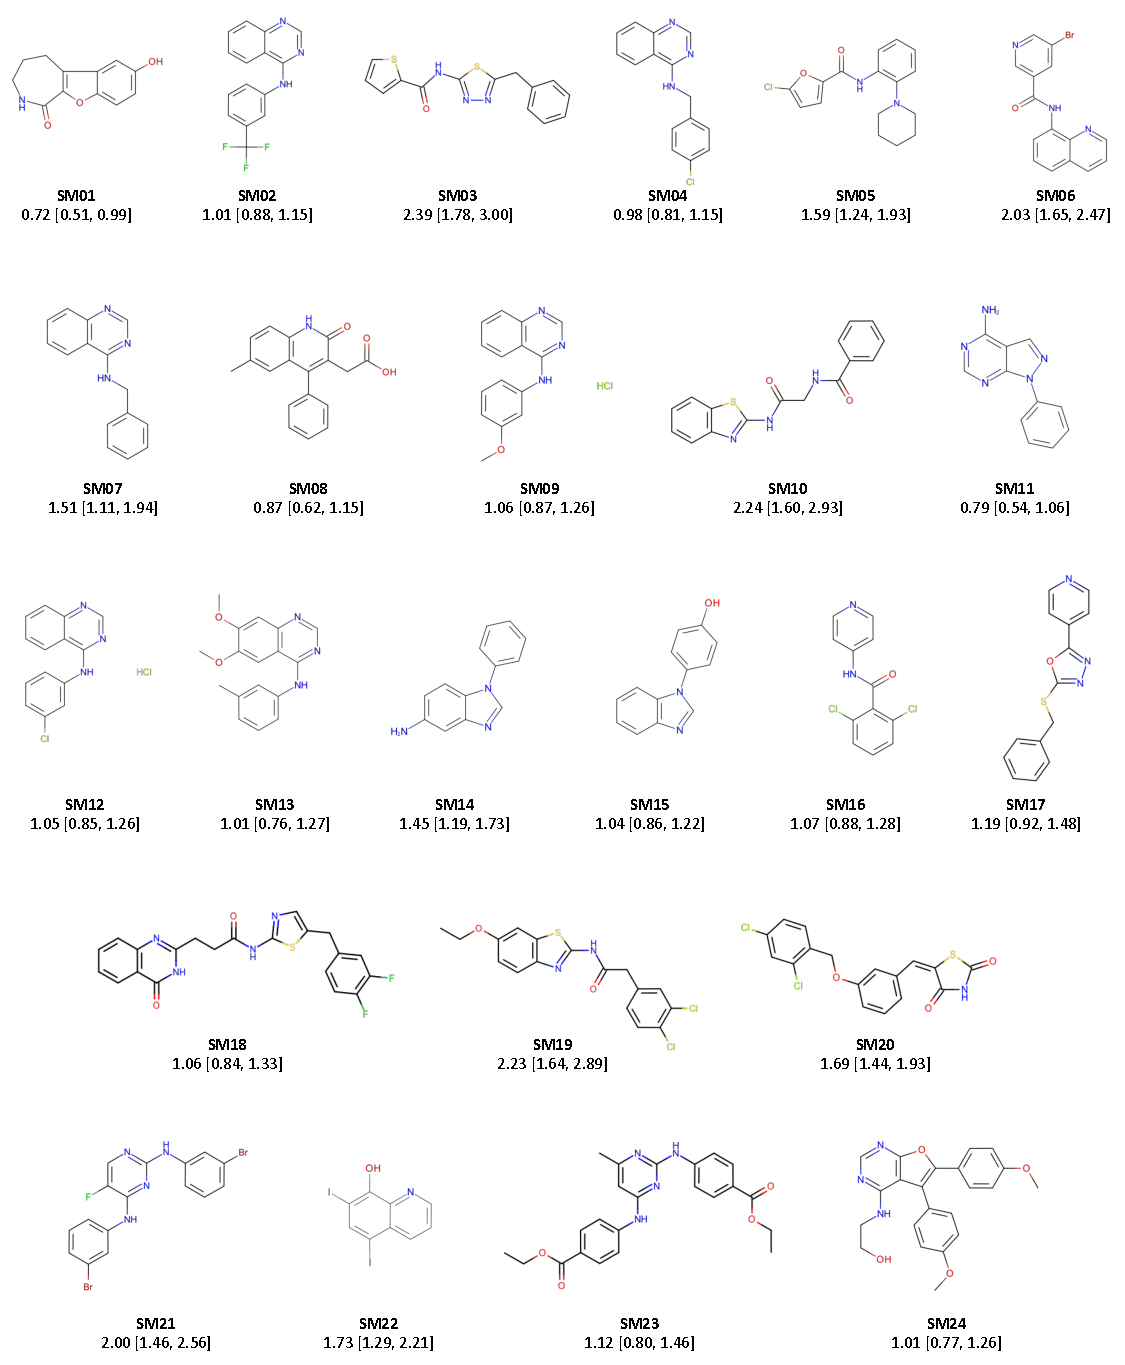
\includegraphics[width=0.95\linewidth]{figures/molecules_with_MAE_of_all_methods.pdf}
\caption{{\bf Molecules of SAMPL6 pKa challenge with MAE calculated for all macroscopic (type III) predictions.} MAE calculated considering all prediction methods indicate which molecules had the lowest prediction accuracy in SAMPL6 challenge. MAE values calculated for each molecule include all the matched pKa values, which could be more than one per method for multiprotic molecules (SM06, SM14, SM15, SM16, SM18, SM22). "C:" and "H:" indicate results based on Closest and Hungarian matching algorithms employed for pairing experimental and predicted pKa values. Calculated MAE values were observed to differ for molecules with multiple experimental pKas. MAE values are reported with 95\% confidence intervals.
\todo[inline]{Add sequencial analysis results to this figure.}
}
\label{fig:molecules_with_MAE_of_all_methods}
\end{center}
\end{figure}

Prediction performance of individual molecules
\todo[inline]{Which chemical structures make pKa predictions more difficult?}
SAMPL6 pKa set consisted of only 24 small molecules which limits our ability to do statistical analysis to determine which chemical substructures contribute to greater errors in pKa predictions.
\todo[inline]{Illustration/explanation of effects where microscopic pKas and macroscopic pKas can differ}

\todo[inline]{Are there any correlations between molecular descriptors and pKa errors?}

\todo[inline]{What can we learn from failures? Which physical effects are driving failures?}




\todoMI{FIGURE:  Molecular MAE comparison across methods.}

Does molecular descriptors explain errors/performance ?
We looked for correlation with descriptors, and potential explanation for errors. Keep spurious correlations in mind if we have many descriptors. No correlation observed. Reference the SI Figure of correlations.

\todo[inline]{Comparison of errors/performance against molecular descriptors. Look for correlation with descriptors, and potential explanation for errors. Keep spurious correlations in mind if we have many descriptors.}

\todoMI{Figure SI: correlation between prediction error and molecular descriptors}

Are pKa predictions better in middle region?
No correlation between pKa value and error was seen.
Reference the SI Figure.

\todoMI{Figure: Ridge plots of Delta pKa error to identify compounds that were frequently mispredicted }

Compare ME of molecules across methods.
Are there molecules often overestimated or underestimated?

No correlation of macroscopic pKa number to the errors? But we have low representation of multiprotic compounds




\subsubsection{Comparing microscopic pKa predictions directly to macroscopic experimental pKa values leads to underestimation of errors}
Discussion of matching experimental and predicted values
\todo[inline]{Difficulty of assessing predicted pKas using experimental data: matching problem}
\todo[inline]{Explain rationale behind how we analyze the data and determine success/failure}

Compare experimental data to microscopic pKa predictions, assuming experimental pKas are titrations of distinguishable sides and therefore equal to microscopic pKas.
Molecules with only 1 pKa or well separated multiple pKas (more than 3 pKa units apart) SM14 and SM18 were excluded from this analysis, since their experimental pKa values don't satisfy these criteria.

Errors computed by microstate-based matching are larger compared to numerical matching algorithms.
Microscopic pKa analysis with numerical matching algorithms may mask errors due to higher number of guesses made.

\todoMI{FIGURE Type I analysis, comparing analysis of 22 molecules (Hungarian vs Microstate matching)}



%%%
\subsection{Analysis of microscopic \pKa{} predictions using microstates determined by NMR (8 molecules)}

\todoMI{FIGURE: Assign experimental pKa to microscopic transitions observed by NMR. }
Conclusions will only be about 4-aminoquinazoline series and benzimidazole (8 molecules, 10 pKas)
Refer to SI figure of dominant microstates.

Choosing molecules with right protonation state is important.
Do people predict the correct sequence of dominant microstates?
 " Even if your pKa prediction is correct, protonation state prediction can be wrong."
 Analyze which state has lowest free energy for each charge group ( The sequence of "experimentally visible states")



\subsubsection{Accuracy of predicted pKa values when microstate matching is used}

\todo[inline]{Assessment of individual methods by each of our analysis methods}
\todo[inline]{Performance comparison of different methods, grouped by methods class}

\todoMI{FIGURE: Ranking of microscopic pKa prediction error statistsics for all participants (8 mol, microstate match).}


\todoMI{FIGURE: Violin plots of Delta pKa error to identify compounds that were frequently mispredicted (microstate match)}



\subsubsection{Dominant microstate prediction accuracy of methods}

Calculate relative free energy of microstates to determine dominant microstate of each charge
Compare predicted and experimental dominant microstates and calculate accuracy of each method

\todoMI{FIGURE: Dominant microstate accuracy vs method plot. Charges together and separate.}

What percent of the time predictions capture the dominant protonation state correctly? 
Match by microstate and calculate RMSE and MAE. If you know the microstates, can you predict the value of the pKa right? 


\todo[inline]{Does top 3 methods predict the same dominant microstate sequence? How differently do different methods predict microscopic transitions? (method vs method correlation plot to see if methods predict the same microstate pairs or not)}


\subsubsection{Which molecules caused lower dominant microstate prediction accuracy?}

Which molecule has more errors in predicting the major microstates?

\todoMI{FIGURE: Dominant micorstate Accuracy vs Molecule ID plot, all charges and separate charges. Also think about plotting  accuracy of QM and empirical methods separately.}


\todo[inline]{Comment on consensus prediction accuracy. Comparison of predicted microstates using consensus set of transitions of high accuracy prediction methods} 


\subsubsection{Demonstrate how numerical matching often masks the error}
Match by Hungarian and calculate accuracy of microstate prediction overall.
When matched by pKa value, do people come with the same transition pairs?

\todoMI{FIGURE: [accuracy-of-microstates-based-on-numeric-matching] For most methods the microstate pair of Hungarian predicted pKa does not match experimentally determined microstate pair.}



%%% 
\subsection{Analyzing microscopic pKa prediction from the perspective of thermodynamics}
Explain  linearity  relative free energy of protonation states with respect to pH. Free energy perspective simplifies data capturing and analysis. Reference Marilyn's paper.

Thermodynamic cycle closure checking allows evaluation of microsopic pKas  without experimental data.
Checking for thermodynamic consistency


\subsubsection{Cycle closure error}

Marilyn observed very good cycle closure results and very bad one that are up to 10 kcal/mol
 
She suggesting checking the cycle with maximum cycle closure error for each method and reporting that for each method.
An historgam of max cycle closure error will help us bin these results into 3 categoris:
1. good agreement
2. moderate
3. severe 
 
"We think thermodyamic cycles of protonation states need to be closed"
Message: Methods need to checked for cycle closure errors.
There can be information there that can be used to correct pKa predictions.
When cycles are not closed it may be used as an indicator of prediction uncertainty.

%%%
\subsection{How would pKa errors affect protein-ligand binding affinity predictions?}

\todo[inline]{How do accuracy limitations in small molecule pKa prediction translate into modeling errors in ligand affinity prediction?}

\todoMI{FIGURE: a diagram illustrating the ways in which the pKa errors can influence prediction errors for binding affinities (A) When minor aqueous protonation state binds (B) When multiple protonation states can bind the complex
}


%%%
\subsection{Lessons learned from SAMPL6 pKa Challenge}
\todo[inline]{Do any methods predict within experimental accuracy (how is the field doing overall)?}
\todo[inline]{Common challenging factors for accurate pKa predictions. Tautomers, Heterocycles etc.}

Overall results:  
Do any methods predict within experimental accuracy (how is the field doing overall)?
Common challenging factors for accurate pKa predictions. Tautomers, Heterocycles etc.

Discussion of matching problem betwene experimental and predicted values.  
Difficulty of assessing predicted pKas using experimental data: matching problem
Explain rationale behind how we analyze the data and determine success/failure.

Conclusion about prediction performance of individual molecules:
SAMPL6 pKa set consisted of only 24 small molecules which limits our ability to do statistical analysis to determine which chemical substructures contribute to greater errors in pKa predictions.  
Which chemical structures make pKa predictions more difficult?  

What can we learn from failures? Which physical effects are driving failures?
Cycle closure errors


%%%
\subsection{Suggestions for future challenges}

\todo[inline]{Discuss what can be done to further improve future challenges}
How can we maximize what we learn?
What should we have people predict?
How should we select compounds / measure pKas?

\todo[inline]{Suggestions about challenge construction}

Enumeration of protonation states before predictions (which states does one need to consider?)

\todo[inline]{Suggestions about challenge analysis}

NMR experimental techniques could be used to validate microstate information in future challenges

Reporting microscopic pKa predictions with charges, microstate free energies is betetr
Experimental dataset with microstate infromation is more helpful.

What can be done to further improve future challenges
How can we maximize what we learn?
What should we have people predict?
How should we select compounds / measure pKas? NMR experimental techniques could be used to validate microstate information in future challenges

Suggestions about challenge construction
Enumeration of protonation states before predictions (which states does one need to consider?)
Suggestions about challenge analysis


%%%%%%%%%%%%%%%%%%%%%%%%%%%%%%%%%%%%%%%%%%%%%%%%%%%%%%%%%%%%














%%%%%%%%%%%%%%%%%%%%%%%%%%%%%%%%%%%%%%%%%%%%%%%%%%%%%%%%%%%%
% Conclusion
%%%%%%%%%%%%%%%%%%%%%%%%%%%%%%%%%%%%%%%%%%%%%%%%%%%%%%%%%%%%
\section{Conclusion}


%%%%%%%%%%%%%%%%%%%%%%%%%%%%%%%%%%%%%%%%%%%%%%%%%%%%%%%%%%%%
% Code and Data Availability
%%%%%%%%%%%%%%%%%%%%%%%%%%%%%%%%%%%%%%%%%%%%%%%%%%%%%%%%%%%%
\section{Code and data availability}
\begin{minipage}{15cm}
\begin{itemize}

\item SAMPL6 \pKa{} challenge instructions, submissions, experimental data and analysis is available at  \href{https://github.com/samplchallenges/SAMPL6}{https://github.com/samplchallenges/SAMPL6}

\end{itemize}
\end{minipage}


%%%%%%%%%%%%%%%%%%%%%%%%%%%%%%%%%%%%%%%%%%%%%%%%%%%%%%%%%%%%
% Overview of supplementary information
%%%%%%%%%%%%%%%%%%%%%%%%%%%%%%%%%%%%%%%%%%%%%%%%%%%%%%%%%%%%
\section{Overview of supplementary information}

\paragraph{Organized in SI document:}

\begin{itemize}
\item TABLE SI 1: ???

\end{itemize}

\paragraph{Extra files:}  
\begin{itemize}
\item Any extra files
\end{itemize}


%%%%%%%%%%%%%%%%%%%%%%%%%%%%%%%%%%%%%%%%%%%%%%%%%%%%%%%%%%%%
% Author Contributions 
%%%%%%%%%%%%%%%%%%%%%%%%%%%%%%%%%%%%%%%%%%%%%%%%%%%%%%%%%%%%
\section{Author Contributions}

Conceptualization, MI, JDC, CB, DLM ; Methodology, MI, JDC ; Software, MI, AR, ASR ; Formal Analysis, MI, ASR, AR ; Investigation, MI ; Resources, JDC;  Data Curation, MI ; Writing-Original Draft, MI, JDC; Writing - Review and Editing, MI, ASR, AR, CB, DLM, JDC; Visualization, MI, AR ; Supervision, JDC, DLM, CB, ASR ; Project Administration, MI ; Funding Acquisition, JDC, DLM.

%(Follow the \href{http://www.cell.com/pb/assets/raw/shared/guidelines/CRediT-taxonomy.pdf}{CRediT Taxonomy})

%%%%%%%%%%%%%%%%%%%%%%%%%%%%%%%%%%%%%%%%%%%%%%%%%%%%%%%%%%%%
% Acknowledgments 
%%%%%%%%%%%%%%%%%%%%%%%%%%%%%%%%%%%%%%%%%%%%%%%%%%%%%%%%%%%%
\section{Acknowledgments}

\todo[inline]{Complete acknowledgments section. Caitlin Bannan, Thomas Fox}
MI, ASR, and JDC acknowledge support from the Sloan Kettering Institute.
JDC acknowledges support from NIH grant P30 CA008748. 
MI acknowledges Doris J.\ Hutchinson Fellowship. 
We thank Brad Sherborne for his valuable insights at the conception of the \pKa{} challenge and connecting us with Timothy Rhodes and Dorothy Levorse who were able to provide resources and expertise for experimental measurements performed at MRL. 
We acknowledge Paul Czodrowski who provided feedback on multiple stages of this work: challenge construction, purchasable compound selection and manuscript. 
MI, ASR, AR and JDC are grateful to OpenEye Scientific for providing a free academic software license for use in this work.

Mike Chui
%\todo[inline]{JDC: Can we cite the ORCIDs of people we thank in this work?}

%%%%%%%%%%%%%%%%%%%%%%%%%%%%%%%%%%%%%%%%%%%%%%%%%%%%%%%%%%%%
% Disclosures 
%%%%%%%%%%%%%%%%%%%%%%%%%%%%%%%%%%%%%%%%%%%%%%%%%%%%%%%%%%%%
\section{Disclosures}

JDC is a member of the Scientific Advisory Board for Schr\"{o}dinger, LLC.
DLM is a member of the Scientific Advisory Board of OpenEye Scientific Software.

Table ref: \cite{ACD-pKa-galas, ACD-pKa-classic, simulation-plus-pKa, chemicalize-pKa, moka-pKa}
trial: [], +, -, *, \#

%%%%%%%%%%%%%%%%%%%%%%%%%%%%%%%%%%%%%%%%%%%%%%%%%%%%%%%%%%%%
%%% BIBLIOGRAPHY
%%%%%%%%%%%%%%%%%%%%%%%%%%%%%%%%%%%%%%%%%%%%%%%%%%%%%%%%%%%%


%\nocite{*} % This command displays all refs in the bib file. PLEASE DELETE IT BEFORE YOU SUBMIT YOUR MANUSCRIPT!
\bibliography{zotero, manual}


%%%%%%%%%%%%%%%%%%%%%%%%%%%%%%%%%%%%%%%%%%%%%%%%%%%%%%%%%%%%
% Supplementary Information
%%%%%%%%%%%%%%%%%%%%%%%%%%%%%%%%%%%%%%%%%%%%%%%%%%%%%%%%%%%%
\newpage
\beginsupplement
\section{Supplementary Information}


\todoMI{Figure [typeIII-error-dist-by-method] Distribution of prediction errors for each method in SAMPL6 Challenge. Analyses was performed based on Hungarian matching algorithm. Y-axis labels indicate submission IDs of each method.}

\todoMI{[pKa-error-vs-pKa-value]. Error in pKa predictions does not correlate with the true value of pKa. Left figure was constructed using closest match between experimental and predicted pKas. Y-axis is absolute residuals of the pKa prediction.}

\todoMI{FIGURE [desc-vs-MAE-correlation]. There is no clear correlation between molecular descriptors and mean absolute error for each molecule when calculated for all methods.
}


\todoMI{ SI Table: Type I collection}
\todoMI{ SI Table: Type III collection}
\todoMI{ SI Figure: type I correlation plots of each method}
\todoMI{ SI Figure: type III correlation plots of each method}


\todoMI{TABLE: InChI and SMILES  for chemicals}
\todoMI{TABLE: Statistics based on hungarian matching}
\todoMI{TABLE: Statistics based on microstate matching}
\todoMI{TABLE: NMR determined microstates of 8 molecules}



\end{document}
